\section{Experiments and Discussions}
\label{sec:experiments}

%We propose a novel sketch-to-face translation model which is robust to hand-drawn sketches. 
Our method is robust to hand-drawn sketches. We conduct extensive experiments to demonstrate the effectiveness of our model in generating high-quality realistic face image from sketches drawn by different users with diverse painting skills.  


\subsection{Implementation Settings}
Before showing experimental results, we first introduce details in our network implementation and training. 


\paragraph{Implementation Details}
We implement our model on Pytorch~\cite{Pytorch}. Both generators for edge-aligned sketches and deformed sketches share an encoder-residual-decoder structure with shared weights except that an SAP module is added to the front of the main generator $G_m$ for deformed sketches. 
The encoder consists of four convolutional layers with $2\times$ downsampling, while the decoder consist of four convolutional layers with $2\times$ upsampling. 
Nine residual blocks between the encoder and decoder enlarge the capacity of the generators. 
%Weights of residual blocks and decoders of two generators share with each other. 
The multi-scale discriminator $D$ consists of three sub-networks for three scales separately, same as Pix2PixHD~\cite{pix2pixHD}. 
Instance normalization~\cite{IN} is applied after the convolutional layers to stabilize training. 
ReLU is used as activation for generators and LeakyReLU for discriminator. 
%
\paragraph{Data}
To produce triplets, consisted of sketches, deform sketches, and real images, $(S, S', x)$ for our network training, we use 
CelebA-HQ~\cite{PGGAN}, a large-scale face image dataset which contains 30K $1024\times1024$ high-resolution face images. 
%
CelebAMask-HQ~\cite{CelebAMask-HQ} offers manually-annotated face semantic masks for CelebA-HQ with 19 classes including all facial components and accessories such as skin, nose, eyes, eyebrows, ears, mouth, lip, hair, hat, eyeglass, earring, necklace, neck, and cloth. We utilize semantic masks in this dataset to extract semantic boundary maps as edge-aligned sketches. 
Deformed sketches are generated by vectorizing and adding random offsets to edge-aligned sketches as discussed in the last section.
Real images, sketches, and deformed sketches are resized to $256\times256$ in our experiments.


\paragraph{Training Details}
All the networks are trained by Adam optimizer~\cite{Adam} with $\beta_1=0.5$ and $\beta_2=0.999$. 
For each training stage, the initial learning rate is set to $0.0002$ and starts to decay at the half of training procedure. 
We set batch size as 32. 
The entire training process takes about three days on four NVIDIA GTX 1080Ti GPUs with 11GB GPU memory.



\paragraph{Baseline Model} 
Pix2pixHD~\cite{pix2pixHD} is a state-of-the-art image-to-image translation model for high-resolution images. 
With the edge-aligned sketches and real face images, we train pix2pixHD with its low-resolution version of generator (`global generator') as a baseline model in our experiment, denoted as \textit{baseline}. 
In order to conduct a fair comparison on generalization, we also train the baseline model with augmented dataset by adding pairs of deformed sketches and images, denoted as \textit{baseline\_deform}.
%
The key idea of our method is using SAP and dual generators to improve the tolerance to sketch distortions. The local enhancer part of pix2pixHD, which is designed for high-resolution image synthesis, can be easily added to improve fine textures for both baseline models and our model in the future. 


\subsection{Quantitative Evaluation on Image Quality}

\subsubsection{Evaluation Metrics} 
Evaluating the performance of generative models has been studied for a period of time in image generation literature.
It is proven to be a complicated task because a model with good performance with respect to one criterion does not necessarily imply good performance with respect to another criterion~\cite{GANs_equal}. 
A proper evaluation metrics should be able to present the joint statistics between conditional input samples and generated images.
Traditional metrics, such as pixel-wise mean-squared error, can not effectively measure the performance of generative models. 
We utilize two popular quantitative perceptual evaluation metrics based on image features extracted by DNNs: Inception Score (IS)~\cite{Improved_Techniques} and Fréchet Inception Distance (FID)~\cite{FID}.
These metrics are proven to be consistent with human perception in assessing the realism of images.

\paragraph{Inception Score (IS)}
IS applies an Inception model pre-trained on ImageNet to extract features of generated images and computes the KL divergence between the conditional class distribution and the marginal class distribution. Higher IS presents higher quality of generative images.
Note that IS is reported to be biased in some cases because its evaluation is based more on the recognizability rather than on the realism of generated samples~\cite{evaluation}. 

\paragraph{Fréchet Inception Distance (FID)}
FID is a recently proposed evaluation metric for generative models and proven to be consistent with human perception in assessing the realism of generated images. FID computes Wasserstein-2 distance between features of generated images and real images which are extracted by a pre-trained Inception model. Lower FID indicates that the distribution of generated data is closer to the distribution of real samples.

%\paragraph{Kernel Inception Distance (KID)}
%KID measures the distance of two distributions by calculating the squared maximum mean discrepancy between Inception features. KID is pointed out as an unbiased estimator with a cubic kernel~\cite{KID}. Lower KIDs indicate better generative models.

%\subsection{Generative Quality with Image Translation Networks}


\subsubsection{Image Quality Comparison}
Existing image-to-image translation models can be trained for sketch-to-face translation using paired sketch and image data. 
Since the quality of generated images presents the basic performance of a generative model, we first compare the quality of generated images by different generative models using IS and FID. 
We test these models with edge-aligned sketches that are synthesized from images in the test set. 
Besides the baseline model, we also test Pix2pix~\cite{pix2pix}, which is the first general image-to-image translation framework. It can be applied to a variety of applications by switching the training data. 
We use the default setting to train Pix2pix model with paired edge-aligned sketches and real face images. 
All these methods produce face image in dimension of $256\times256$.

Table~\ref{tab:generative_quality} shows the quantitative evaluation results of four models. Our model surpasses other models by a small margin with respect to two evaluation metrics. 
Visual results are shown in Figure~\ref{fig:generative_quality}. As we can see, all of the four models are able to generate plausible face images from sketches of test dataset. Since these test sketches are generated using the same method as training sketches, the test data distribution is quite close to/overlapped with the training data distribution. Both our model and existing models are easily to be generalize to handle these samples. We will show our model's superiority on generalization to more challenging sketches in the next few experiments.



\begin{table}[h]
	\centering	
	\caption{Results of generative quality comparison.}
	\begin{tabular}{|c|c|c|c|c|}\hline
		& Pix2pix \cite{pix2pix} & Baseline~\cite{pix2pixHD} & Baseline\_deform & Ours \\\hline
		IS & $2.186$ & $2.298$ & $2.369$ & $\textbf{2.411}$\\\hline
		FID & $289.3$ & $259.1$ & $244.3$ & $\textbf{242.1}$\\\hline
	\end{tabular}
	\label{tab:generative_quality}
\end{table} 

\begin{figure}
	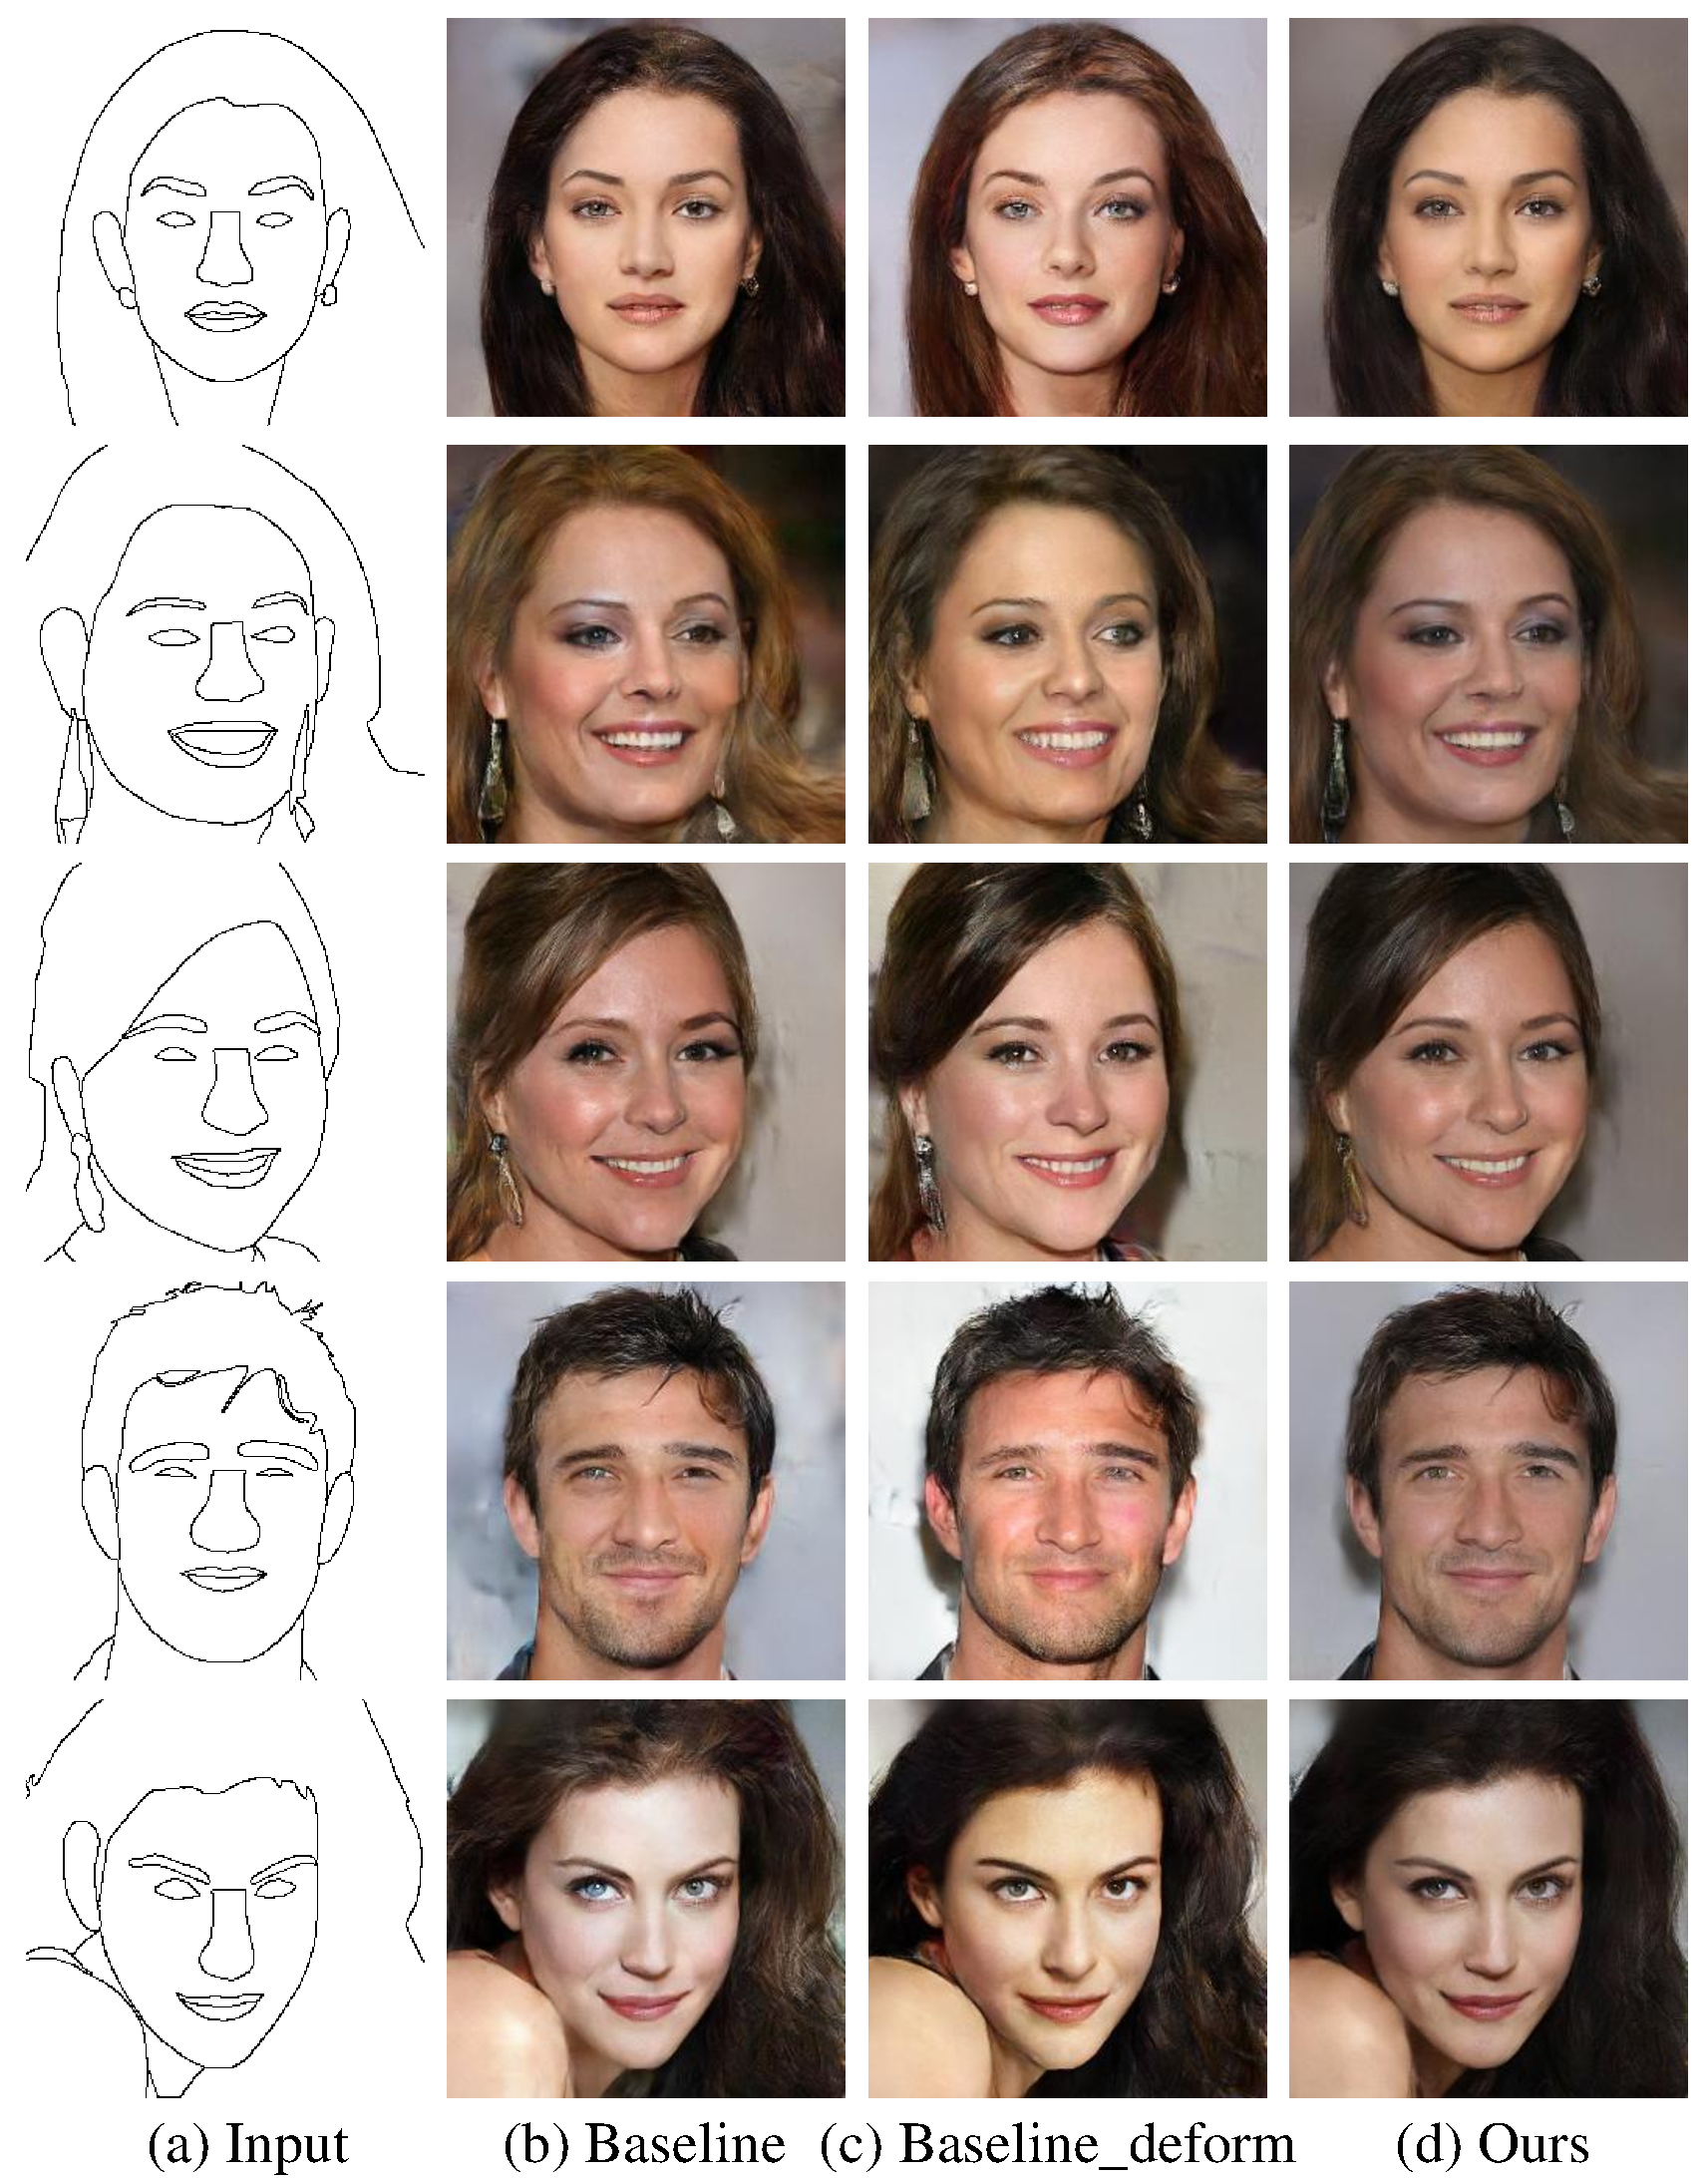
\includegraphics[width=0.9\linewidth]{figs/results}
	\caption{Both our model and existing models, which generate plausible photo-realistic face images from sketches in test set, are able to be generalized to test sketches from similar distribution as the training distribution. We will show our model's superiority on generalization to more challenging sketches in the next few experiments.}
	\label{fig:generative_quality}
\end{figure}

\subsection{Comparison of Generalization Capability}

In order to verify the generalization ability of our model, we compare our model with state-of-the-art image translation models by testing with synthesized sketches of different levels of deformation, well-drawn sketches and poorly-drawn sketches by novel users.

\subsubsection{Different Level of Deformation}
As mentioned in Subsection~\ref{subsec:algorithm_data}, we deform an edge-aligned sketch $S$ to obtain a corresponding deformed sketch $S'$ by adding random offsets to the control points and end points of the vectorized strokes in $S$. 
The maximum offset $d$ is set to $11$ in the training data. 
We further create more deformed sketches with multiple levels of deformation, denoted as $S'_d$, by modifying the maximum offset $d$.
%
We examine the generalization ability of our model and baseline model on these deformed sketches. 
Note that the \textit{baseline} is trained with only edge-aligned sketches while our model and \textit{baseline\_deform} model are trained both edge-aligned sketches and deformed sketches with $d=11$.

In this experiment, the input sketches are deformed by larger offsets where the maximum $d$ is set to $30$. 
As shown in Figure~\ref{fig:generalization_examples}, strokes in sketches with larger deformation looks quite different from those in the training sketches including edge-aligned sketches $S$ and deformed sketches $S_{11}'$. 
%
By adding deformed sketches into training data, \textit{baseline\_deform} produces better images than \textit{baseline}. However, when larger deformation occurs, \textit{baseline\_deform} suffers from artifacts in facial features, for example, the mouth in the first example, the eyes of the third and the last case in Figure~\ref{fig:generalization_examples}, 
In comparison, our model produces more realistic face images with more symmetric eyes and find textures, benefited from its ability of capturing shape feature from deformed strokes by our spatial attention pooling module. 
\begin{figure}
	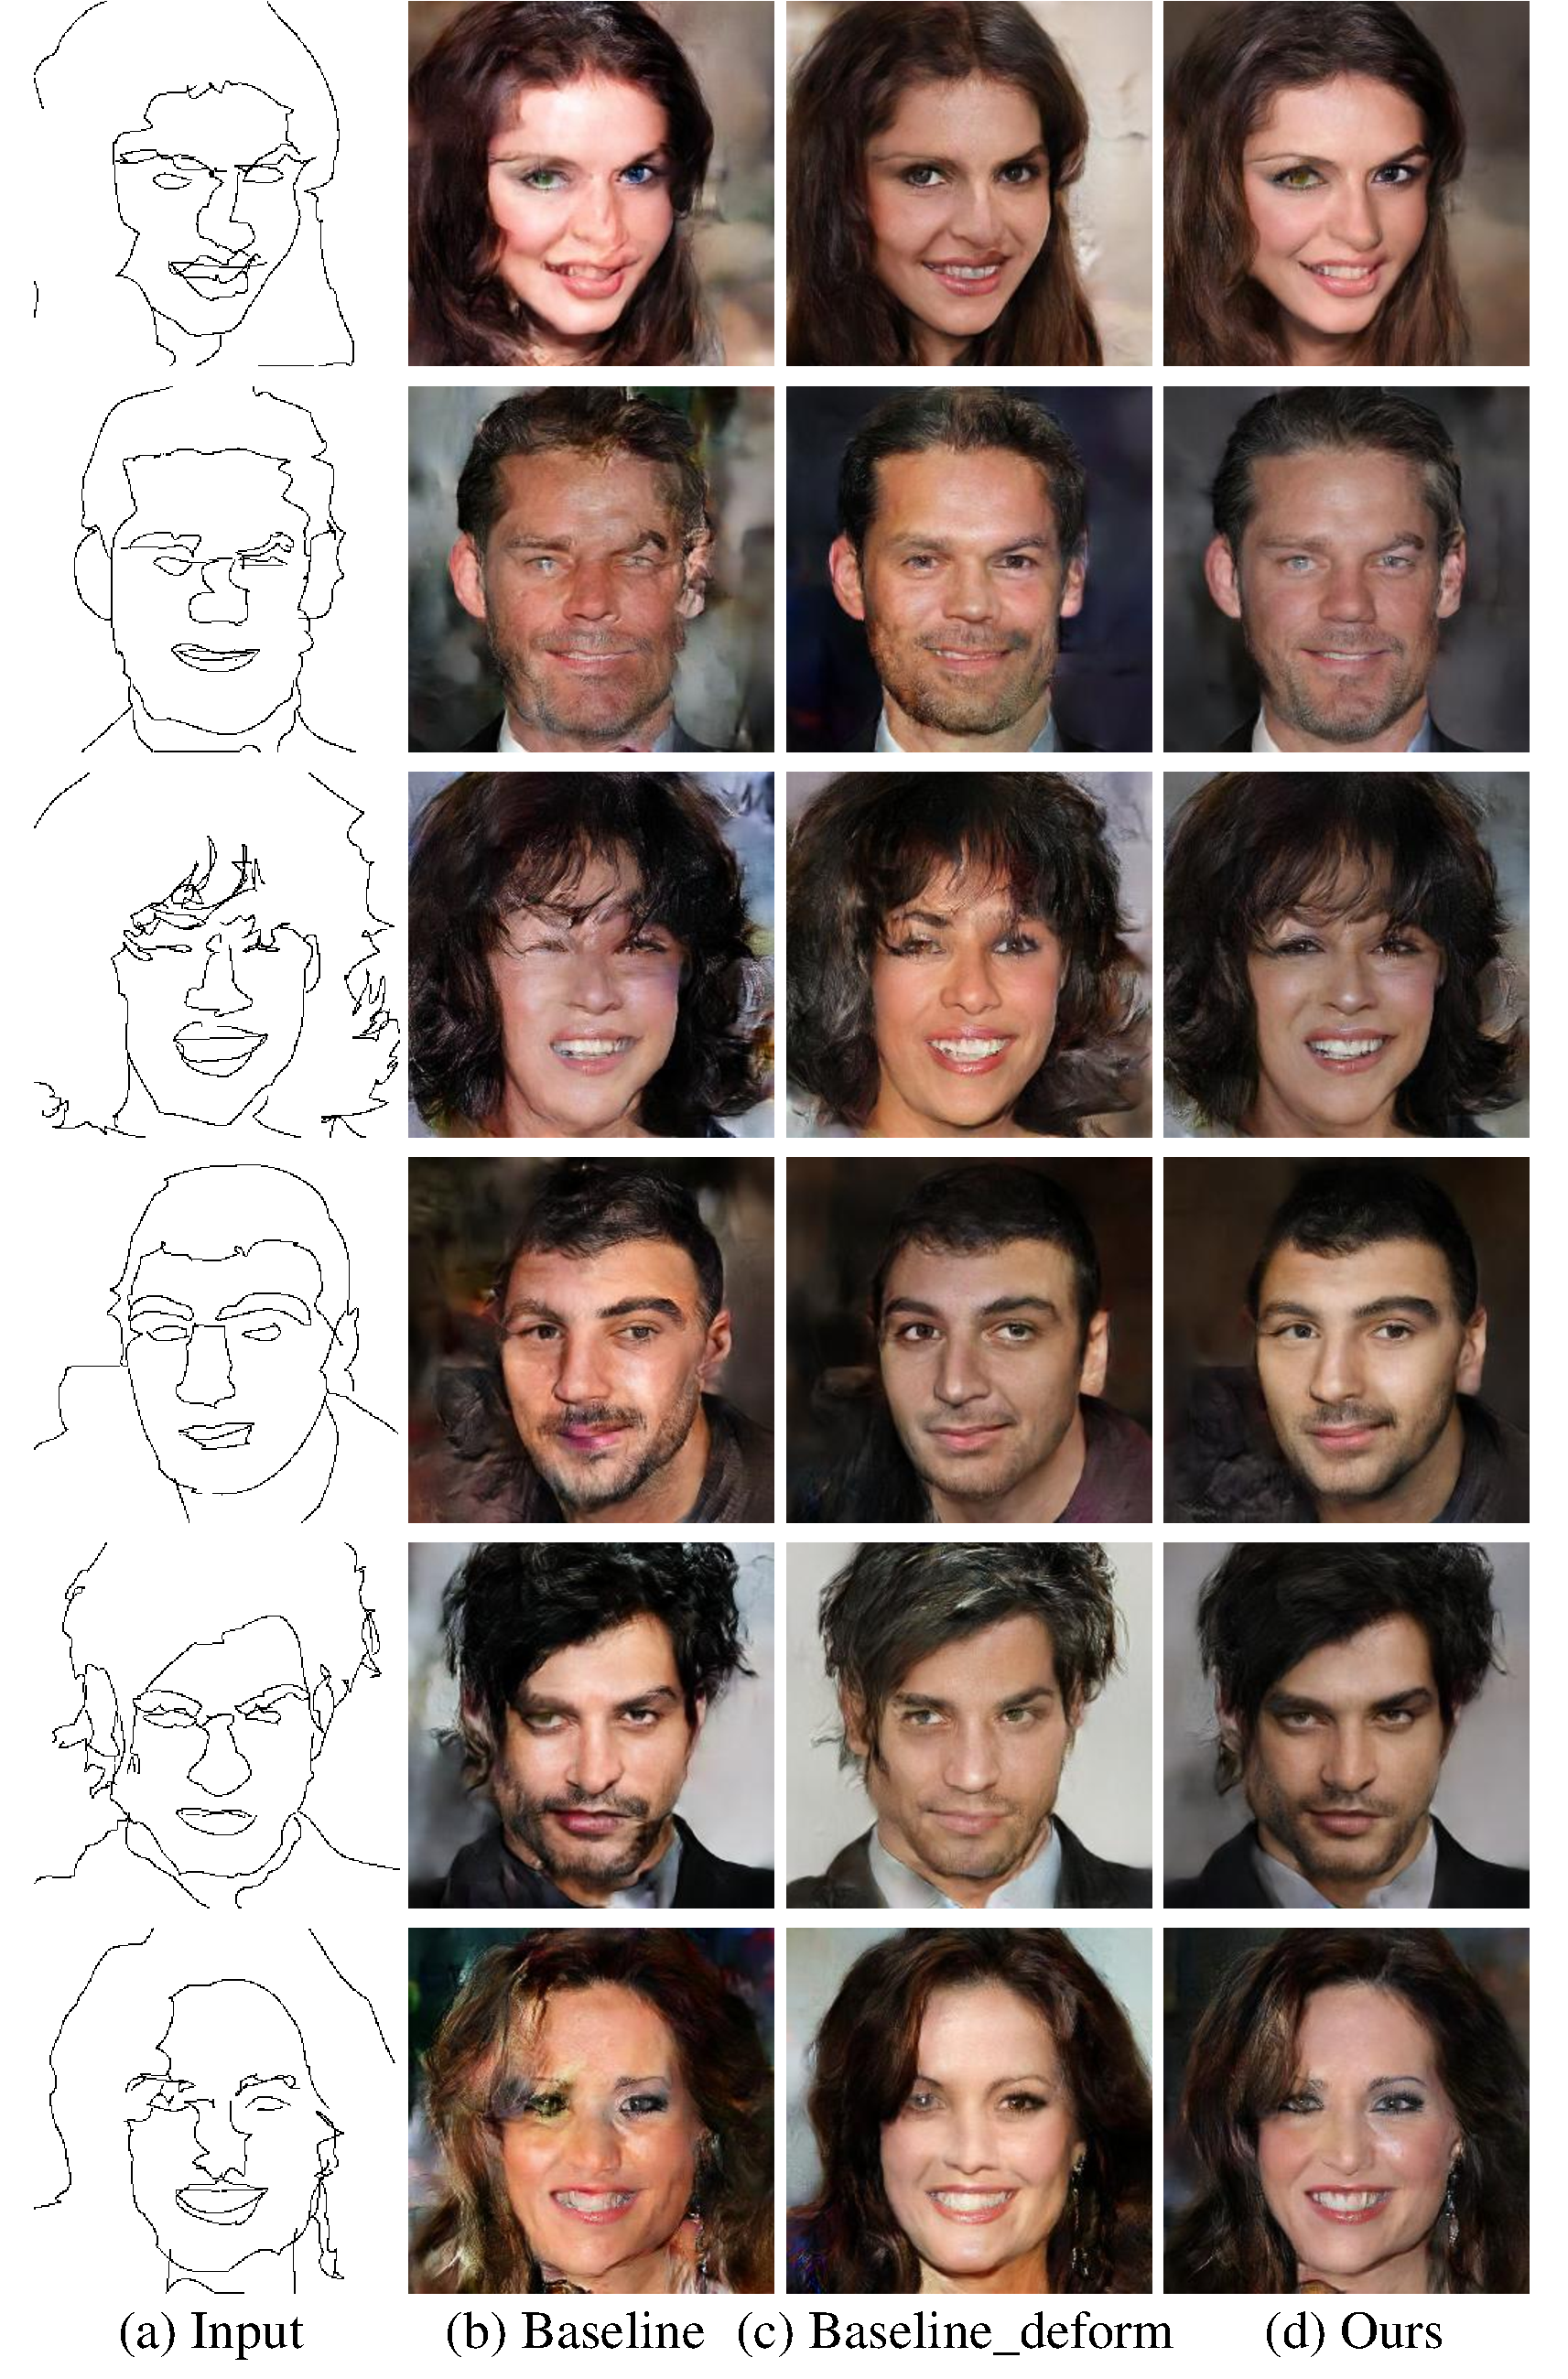
\includegraphics[width=0.9\linewidth]{figs/generalization_examples}
	\caption{For sketches with large deformation, both \textit{baseline} model and \textit{baseline\_deform} model fail to generate satisfying results, in which artifacts can be found in areas with large sketch deformation. Our results maintain high quality even large deformation occurs.  }
	\label{fig:generalization_examples}
\end{figure}

\subsubsection{Hand-Drawn Sketches}
Besides the synthesized sketches with stroke deformation, we further examine the model generalization ability by comparing performances of our model with baseline model tested with two kinds of hand-drawn sketches: expert-drawn sketches and common-user sketches drawn by users without professional painting skills.

\paragraph{Expert-Drawn Sketches}
We invite an expert with well-trained drawing skills to draw portrait sketches for testing. 
These expert sketches were drawn on a pen tablet so that the strokes are smooth and precise. 
Note that shading strokes are not drawn. 
%
Figure~\ref{fig:expert_sketches} shows a group of face images generated by different models from several expert-drawn sketches. 
%
Even with well-drawn strokes, the \textit{baseline} and \textit{baseline\_deform} frequently fail to produce realistic textures and complete structures of eyes or mouths. 
%
In comparison, our results are more realistic with fine textures and intact structures. 

\begin{figure}
	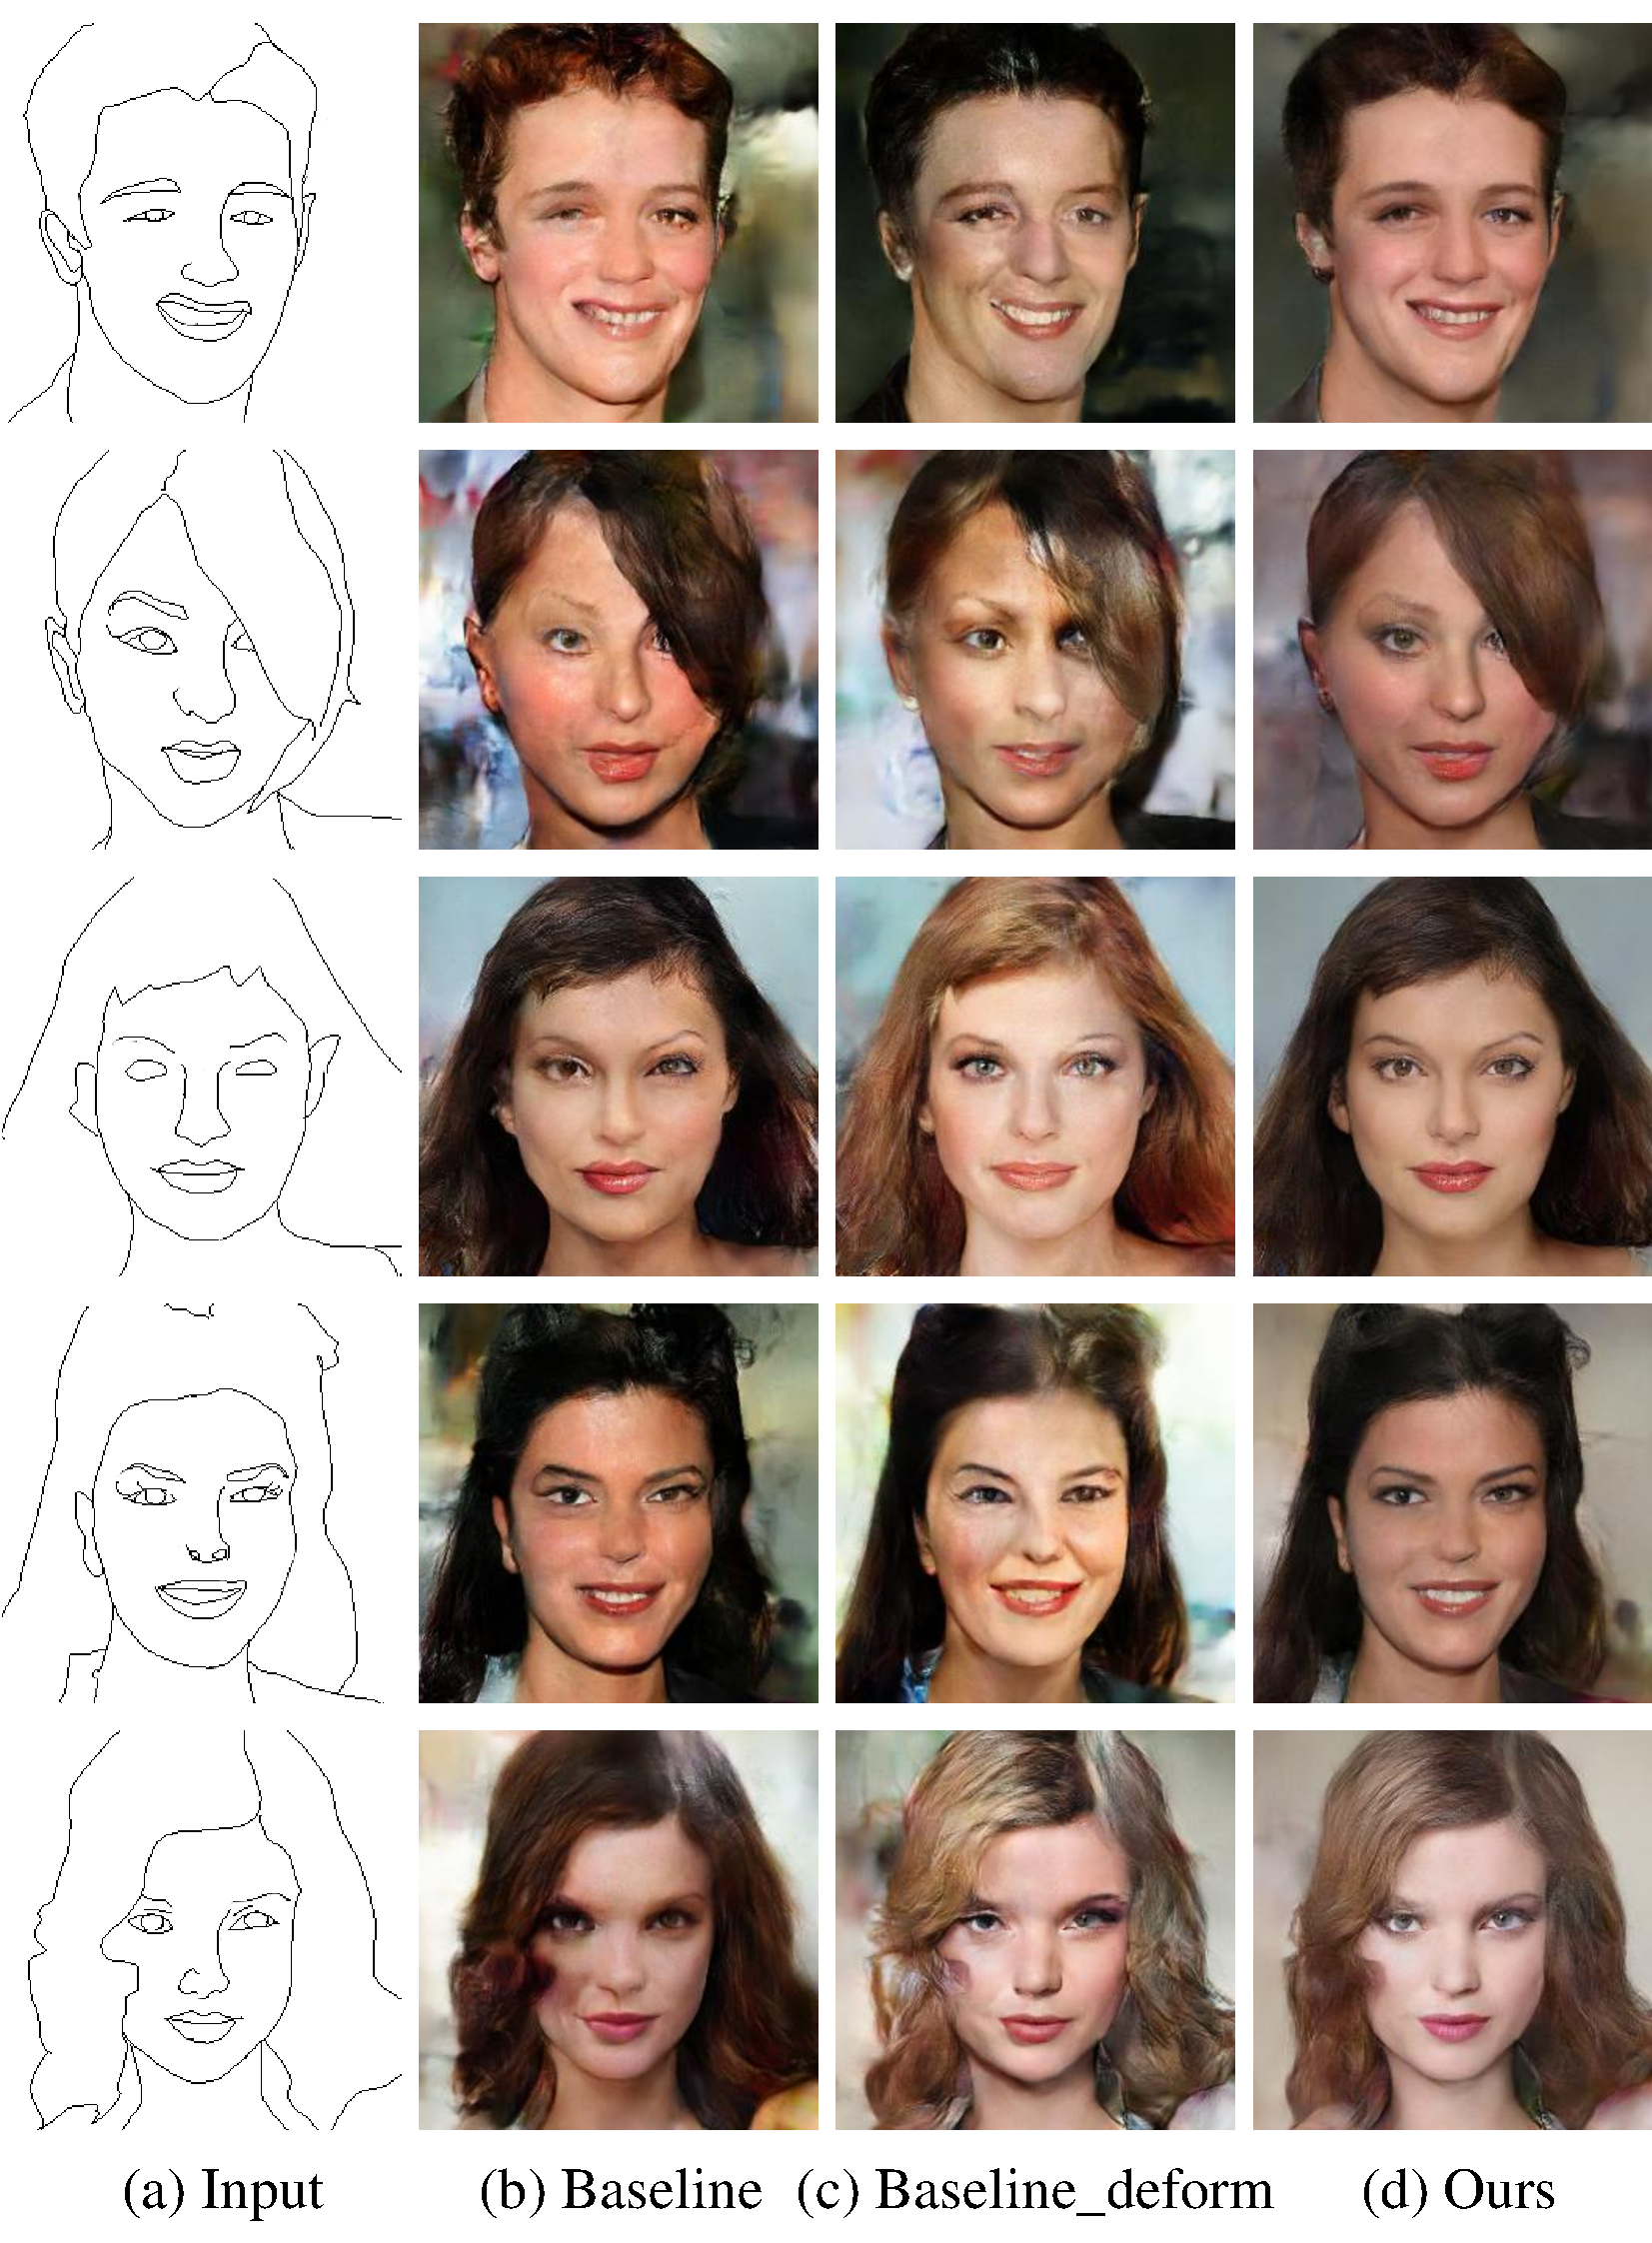
\includegraphics[width=0.9\linewidth]{figs/expertsketches}
	\caption{Our model is able to be generalized to well-drawn expert sketches while results of baseline models are degenerated.}
	\label{fig:expert_sketches}
\end{figure}


\paragraph{Common Sketches}
We also invited a large number of graduate students without drawing skills to draw freehand sketches of their imagined faces using mouses. Hence, strokes of these common sketches rough depicts the desired face structure and shapes of facial features with some distortion. 
Moreover, common sketches turn to be of different levels of details. For example, some sketches contains many strokes inside the hair areas which are blank in the training sketches. 
%
Results shown in Figure~\ref{fig:common_sketches} demonstrate that our model is robust to these poorly-drawn sketches. 
In constrast, the diversity of stroke styles and detail levels significantly damage the quality of the results from the \textit{baseline} model and \textit{baseline\_deform} model.


\begin{figure}
	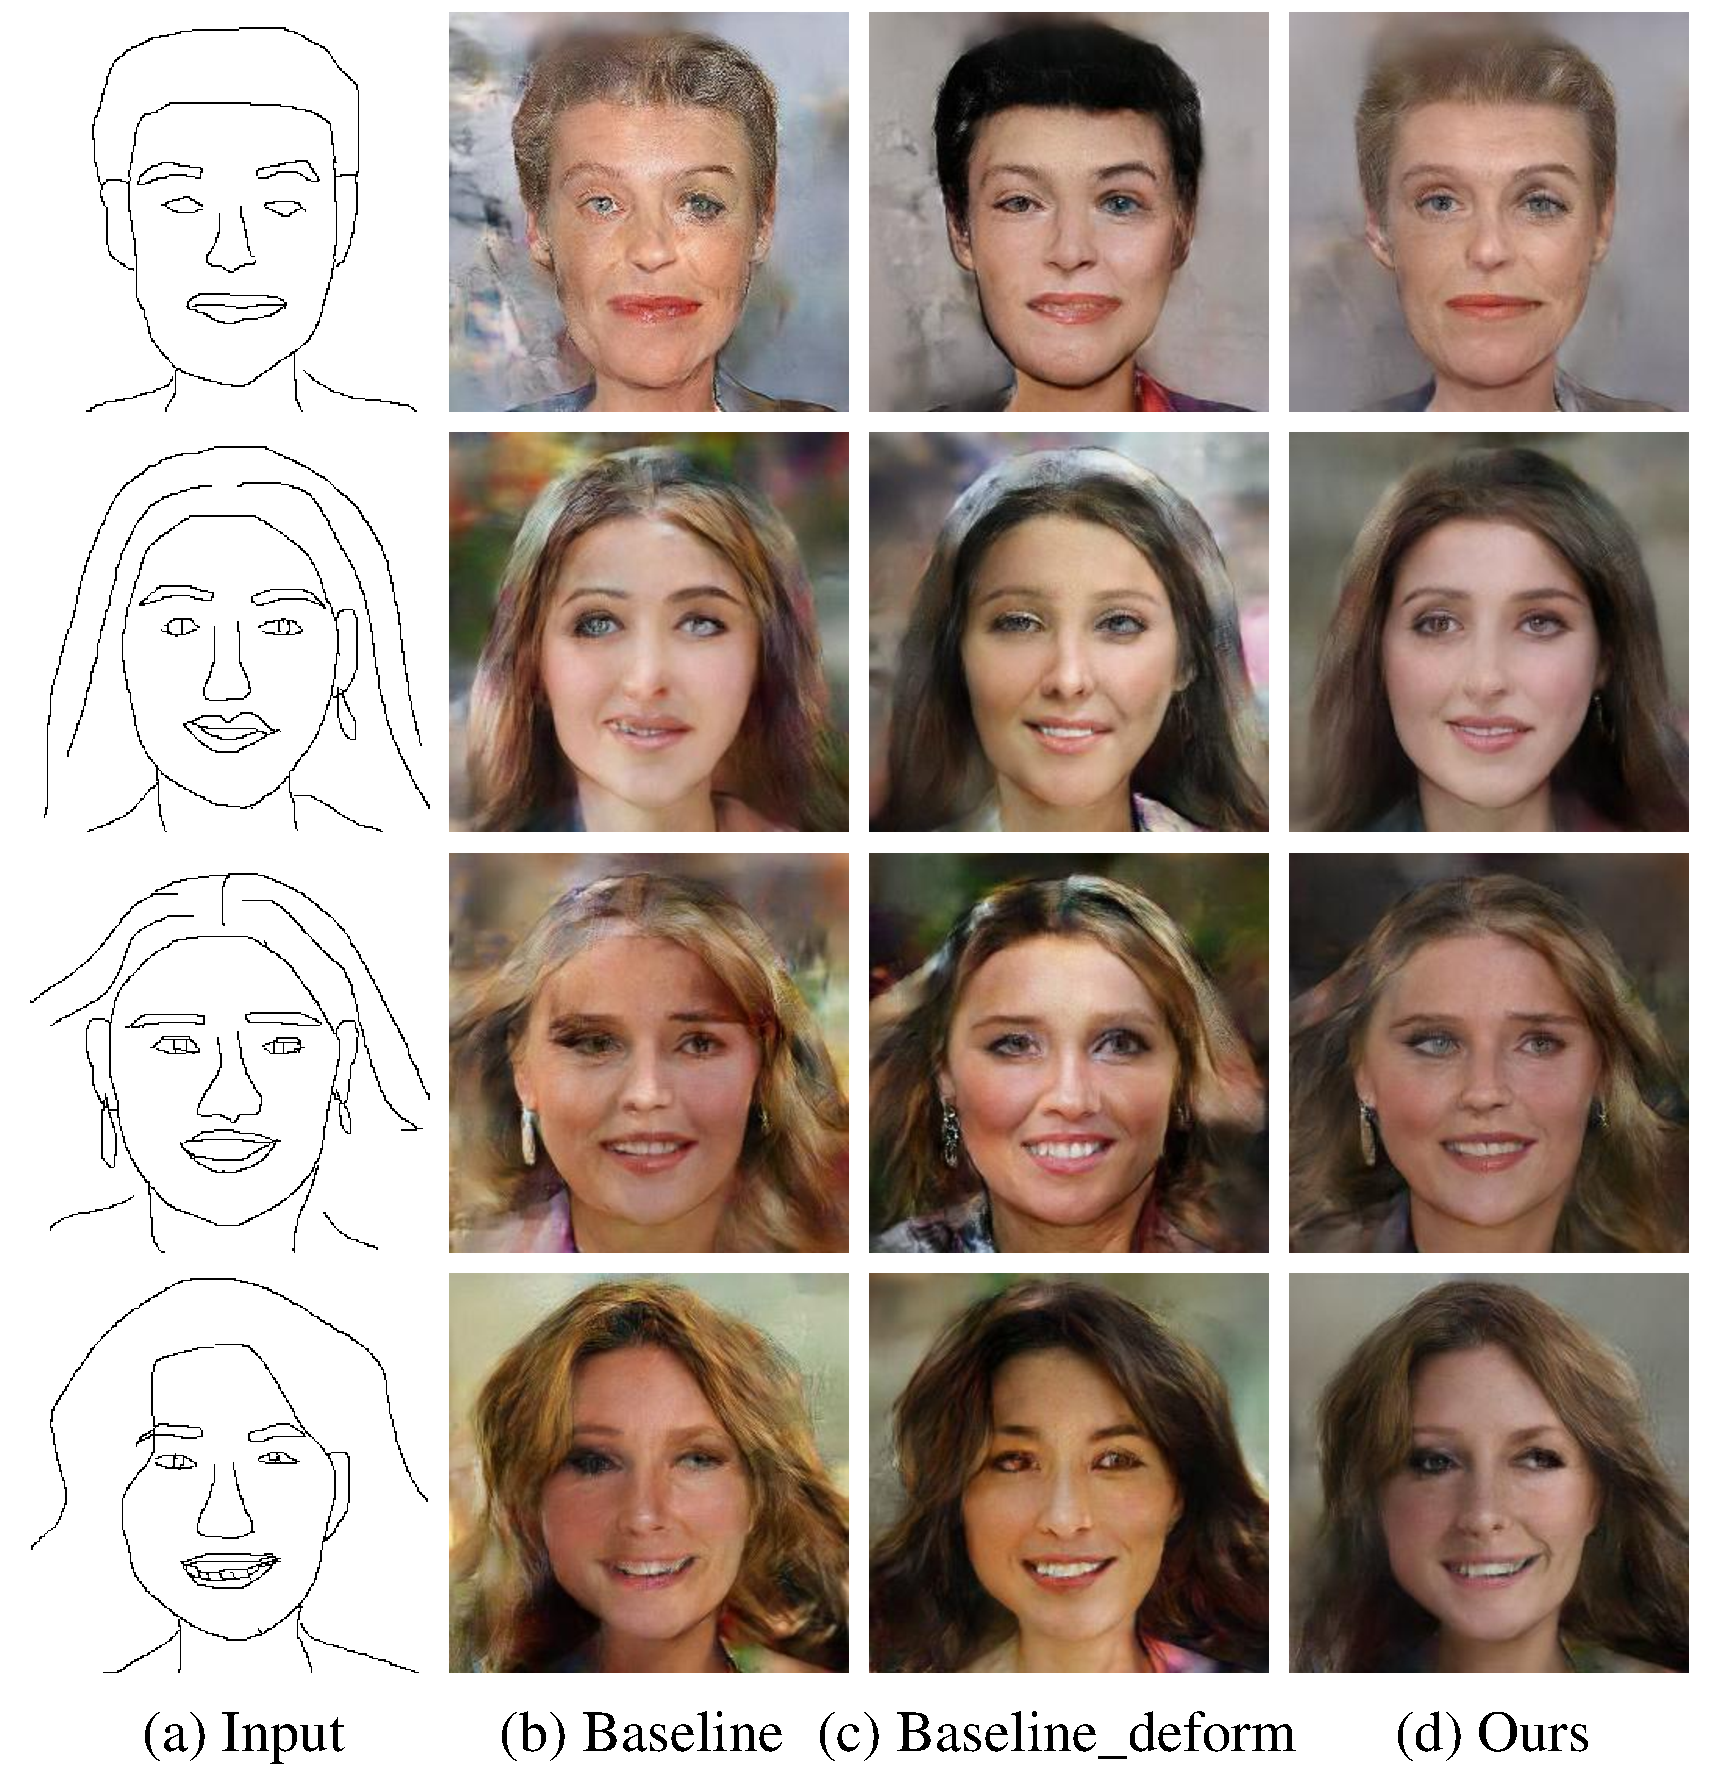
\includegraphics[width=0.9\linewidth]{figs/commonsketches}
	\caption{For these challenging sketches drawn by common users, our model still generate plausible results. Results of baseline models are over-blurred and contains obvious artifacts.}
	\label{fig:common_sketches}
\end{figure}

